\documentclass[12pt]{article}
\usepackage[margin=0.7in]{geometry}
\usepackage{graphicx}
\usepackage{amsmath}
\usepackage{float}
\usepackage{capt-of}
\usepackage{varwidth}
\usepackage{booktabs}

% Define a command to layout a table
% Inpute values are #1 input layer bias node
%                   #2 hidden layer bias node
%                   #3 standardization of features
%                   #4 PCA applied
%                   #5 Testing Accuracy
%                   #6 Table Caption
\newcommand{\testingAccuracyTable}[6] {
  \begin{tabular}{l|l}
    \hline
    Input layer bias node & #1 \\
    Hidden layer bias node & #2 \\
    Standardization of features & #3 \\
    PCA applied & #4 \\
    \hline
    Testing Accuracy & #5 \\
    \hline
  \end{tabular}
  ~\\[60pt]
  \caption{#6}
}

% Define a command to layout a table and plot
% Inpute values are #1 input layer bias node
%                   #2 hidden layer bias node
%                   #3 standardization of features
%                   #4 PCA applied
%                   #5 Testing Accuracy
\newcommand{\testingAccuracyTableAndPlot}[5] {
  \begin{center}
    \begin{table}[H]
      \begin{varwidth}[b]{0.4\linewidth}
        \centering
        \testingAccuracyTable{#1}{#2}{#3}{#4}{#5}{#1#2#3#4 Testing Accuracy}
        \label{table:#1#2#3#4}
      \end{varwidth}%
      \hfill
      \begin{minipage}[b]{0.6\linewidth}
        \centering
        \includegraphics[width=100mm]{./accuracy_imgs/#1#2#3#4_training_accuracy.png}
        \captionof{figure}{#1#2#3#4 Training Accuracy}
        \label{fig:#1#2#3#4}
      \end{minipage}
    \end{table}
  \end{center}
}

\begin{document}

\begin{titlepage}

\newcommand{\HRule}{\rule{\linewidth}{0.5mm}} % Defines a new command for the horizontal lines, change thickness here

\center % Center everything on the page

%----------------------------------------------------------------------------------------
%	HEADING SECTIONS
%----------------------------------------------------------------------------------------

\textsc{\LARGE Drexel University}\\[1.5cm] % Name of your university/college
\textsc{\Large CS499I}\\[0.5cm] % Major heading such as course name
\textsc{\large Advanced Neural Networks}\\[0.5cm] % Minor heading such as course title

%----------------------------------------------------------------------------------------
%	TITLE SECTION
%----------------------------------------------------------------------------------------

\HRule \\[0.4cm]
{ \huge \bfseries Facial Recognition With Artificial Neural Networks}\\[0.4cm] % Title of your document
\HRule \\[1.5cm]

%----------------------------------------------------------------------------------------
%	AUTHOR SECTION
%----------------------------------------------------------------------------------------

\begin{minipage}{0.4\textwidth}
\begin{flushleft} \large
\emph{Author:}\\
Alexander \textsc{Marion}\\
Matthew \textsc{D'Amore}
\end{flushleft}
\end{minipage}
~
\begin{minipage}{0.4\textwidth}
\begin{flushright} \large
\emph{Supervisor:} \\
Dr. Matthew \textsc{Burlick}
\end{flushright}
\end{minipage}\\[4cm]

% If you don't want a supervisor, uncomment the two lines below and remove the section above
%\Large \emph{Author:}\\
%John \textsc{Smith}\\[3cm] % Your name

%----------------------------------------------------------------------------------------
%	DATE SECTION
%----------------------------------------------------------------------------------------

{\large \today}\\[3cm] % Date, change the \today to a set date if you want to be precise

%----------------------------------------------------------------------------------------
%	LOGO SECTION
%----------------------------------------------------------------------------------------

%\includegraphics{Logo}\\[1cm] % Include a department/university logo - this will require the graphicx package

%----------------------------------------------------------------------------------------

\vfill % Fill the rest of the page with whitespace
\end{titlepage}

\newpage

\section{Datasets}
\textbf{Yale Faces Database} \quad This dataset contains 165 grayscale images in GIF format of 15 individuals with 11 images per person. There is one image per each of the following configurations: center-light, w/glasses, happy, left-light, w/no glasses, normal, right-light, sad, sleepy, surprised, and wink.

\section{Testing Parameters}
The following variants are tested for accuracy:
\begin{enumerate}
  \item With and without a bias node at the input layer
  \item With and without a bias node at the hidden layer
  \item With and without standardizing features
  \item With and without applying PCA to reduce the number of features to 95\%
\end{enumerate}
Empirical data was generated to optimize the following parameters:
\begin{enumerate}
  \item Termination criteria (Number of Training Iterations)
  \item Hidden layer size
  \item Image size
  \item Learning Rate
  \item PCA Field Retention
\end{enumerate}

\section{Baseline Accuracy}
The baseline accuracy was created using the negative form of all variants with the exception of data standardization. The baseline parameters were as follows: 40 by 40 sized images, a hidden layer size of 20, 1000 training iterations, and a learning rate of 0.5.
\begin{center}
  \begin{table}[H]
    \begin{varwidth}[b]{0.4\linewidth}
      \centering
      \testingAccuracyTable{N}{N}{Y}{N}{0.800000}{Baseline Testing Accuracy}
      \label{table:baseline}
    \end{varwidth}%
    \hfill
    \begin{minipage}[b]{0.6\linewidth}
      \centering
      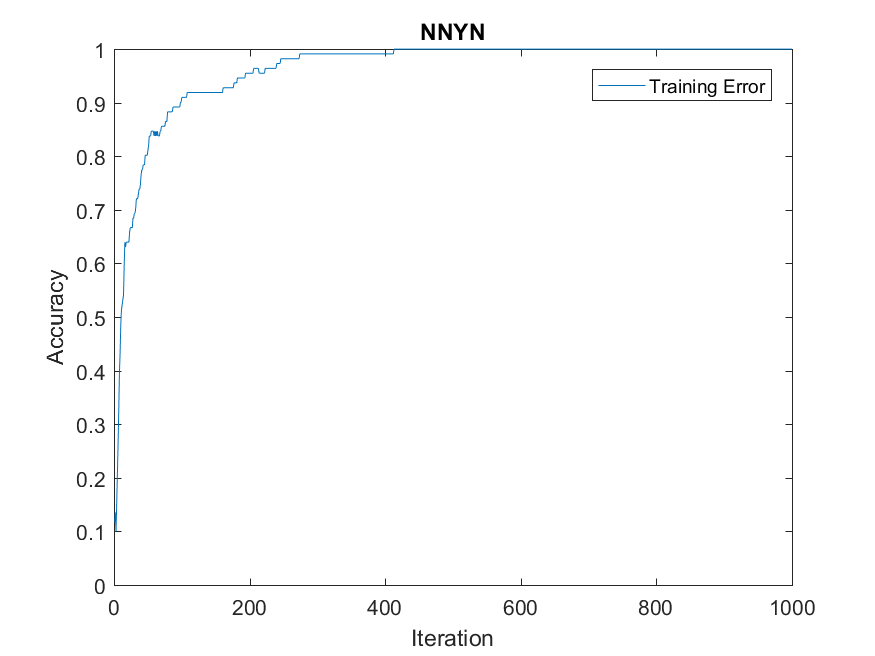
\includegraphics[width=100mm]{accuracy_imgs/baseline_training_accuracy.png}
      \captionof{figure}{Baseline Training Accuracy}
      \label{fig:baseline_img}
    \end{minipage}
  \end{table}
\end{center}

\section{Variant Accuracy Testing}
All variants were tested using 40 by 40 sized images, a hidden layer size of 20, 1000 training iterations, a learning rate of 0.5, and a PCA retention rate of 0.95.

\testingAccuracyTableAndPlot{N}{N}{N}{N}{0.163636}
\testingAccuracyTableAndPlot{Y}{N}{N}{N}{0.272727}
\testingAccuracyTableAndPlot{N}{Y}{N}{N}{0.218182}
\testingAccuracyTableAndPlot{N}{N}{N}{Y}{0.254545}
\testingAccuracyTableAndPlot{Y}{Y}{N}{N}{0.200000}
\testingAccuracyTableAndPlot{Y}{N}{Y}{N}{0.818182}
\testingAccuracyTableAndPlot{Y}{N}{N}{Y}{0.163636}
\testingAccuracyTableAndPlot{N}{Y}{Y}{N}{0.836364}
\testingAccuracyTableAndPlot{N}{Y}{N}{Y}{0.309091}
\testingAccuracyTableAndPlot{N}{N}{Y}{Y}{0.945455}
\testingAccuracyTableAndPlot{Y}{Y}{Y}{N}{0.781818}
\testingAccuracyTableAndPlot{Y}{Y}{N}{Y}{0.327273}
\testingAccuracyTableAndPlot{Y}{N}{Y}{Y}{0.963636}
\testingAccuracyTableAndPlot{N}{Y}{Y}{Y}{0.945455}
\testingAccuracyTableAndPlot{Y}{Y}{Y}{Y}{0.945455}

\newpage
\section{Empirical Parameter Accuracy Testing}
All empirical data was gathered using the following variant which had the highest accuracy from the variant testing:
\testingAccuracyTableAndPlot{Y}{N}{Y}{Y}{0.963636}

\begin{enumerate}
  \item Number of Training Iterations
  The number of training iterations was varied from 0 to 10,000 by 100. The number of hidden nodes was 20, the image size was 40 by 40, and the learning rate was 0.5. The following is a plot of the accuracy as number of training iterations increases.
  \begin{center}
    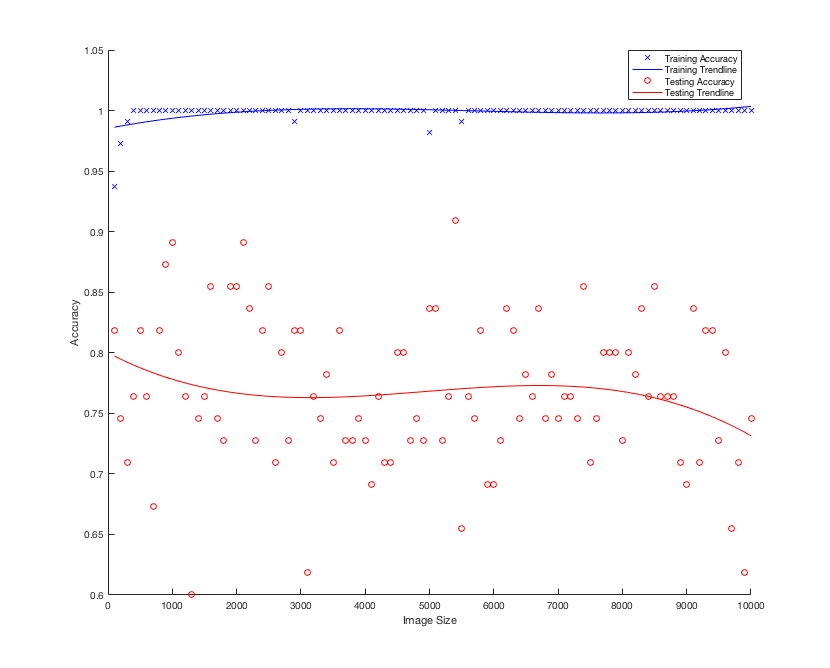
\includegraphics[width=115mm]{./accuracy_imgs/num_iterations_empirical.png}
    \captionof{figure}{Plot of accuracy as number of training iterations increases}
    \label{fig:num_iterations}
  \end{center}
  \item Number of Hidden Nodes
  The number of hidden nodes was varied from 0 to 1600 (the number of features) by 20. The number of training iterations was 10, the image size was 40 by 40, and the learning rate was 0.5. The following is a plot of the accuracy as number of hidden nodes increases. The number of training iterations was reduced to 10 in order to more clearly show the trend of increasing the number of hidden nodes.
  \begin{center}
    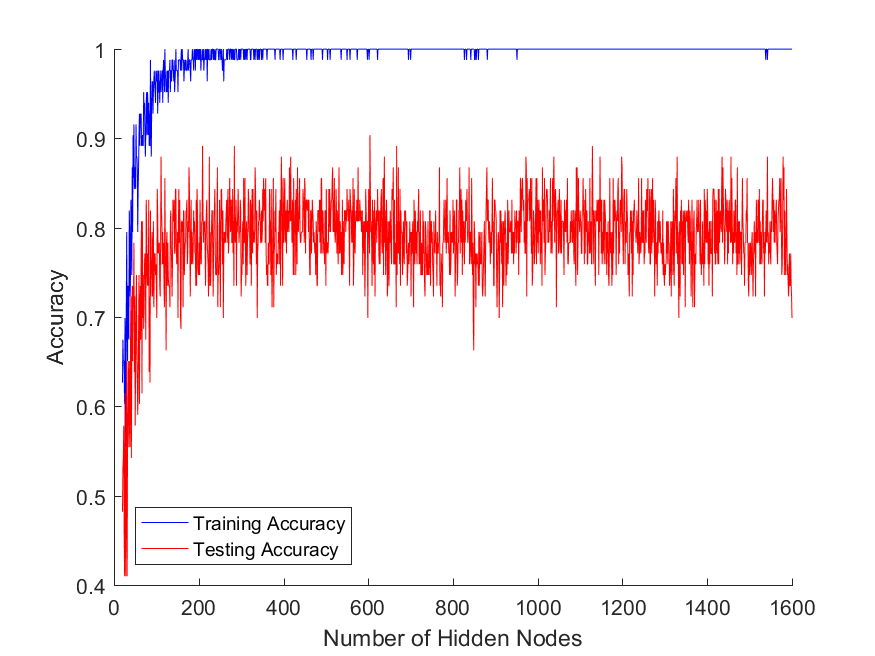
\includegraphics[width=115mm]{./accuracy_imgs/num_hidden_nodes_empirical.png}
    \captionof{figure}{Plot of accuracy as number of hidden nodes increases}
    \label{fig:num_hidden_nodes}
  \end{center}
  \item Image Size
  The image size was varied from 10 to 100 by 1, thus increasing the number of features quadratically. The number of training iterations was 500, the number of hidden nodes was 20, and the learning rate was 0.5. The number of training iterations was reduced to 500 in order to more clearly show the trend of increasing the number of hidden nodes.
  \begin{center}
    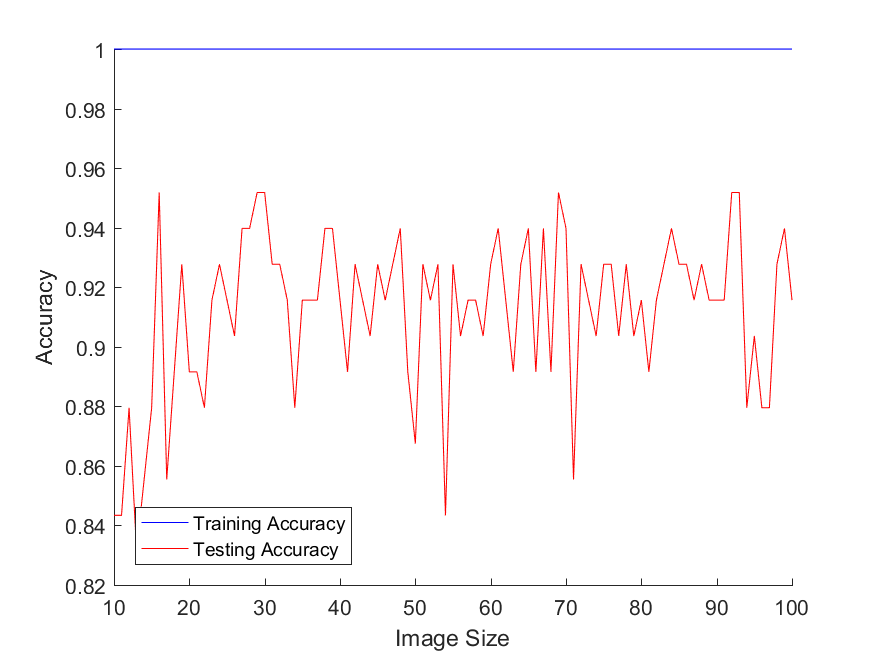
\includegraphics[width=115mm]{./accuracy_imgs/image_size_empirical.png}
    \captionof{figure}{Plot of accuracy as the image size increases}
    \label{fig:img_size}
  \end{center}
  \item Learning Rate
  The learning rate was varied from 0.05 to 20 by 0.05. The number of training iterations was 50, the number of hidden nodes was 20, and the image size was 40 by 40. The number of iterations was reduced to 50 in order to more clearly show the trend of increasing the learning rate.
  \begin{center}
    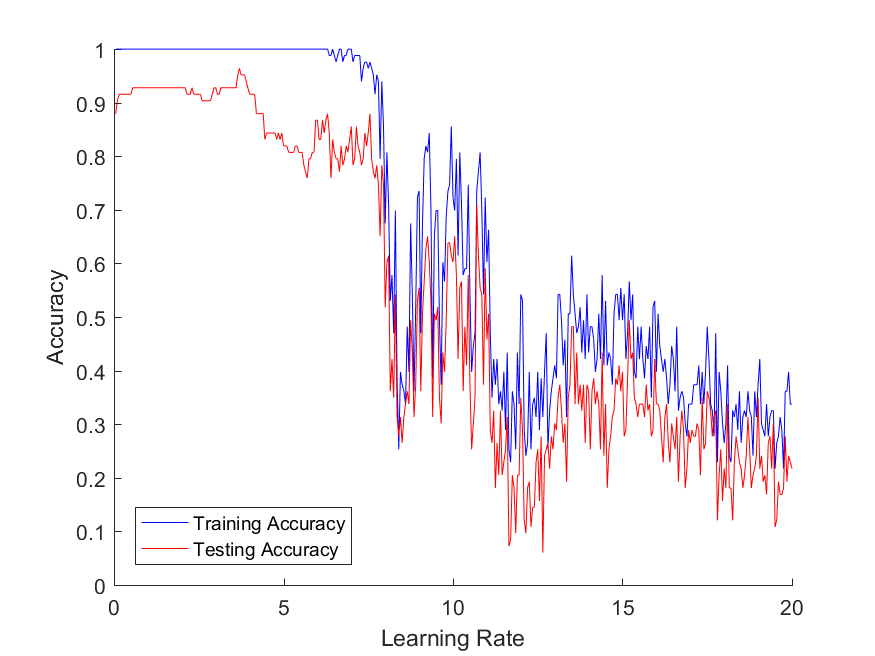
\includegraphics[width=115mm]{./accuracy_imgs/learning_rate_empirical.png}
    \captionof{figure}{Plot of accuracy as the learning rate increases}
    \label{fig:img_size}
  \end{center}
  \item PCA Field Retention
  The PCA field retention rate was varied from 0.01 to 1 by 0.01. The number of training iterations was 200, the number of hidden nodes was 20, and the image size was 40 by 40. The number of iterations was reduced to 200 in order to more clearly show the trend of increasing the PCA field retention.
  \begin{center}
    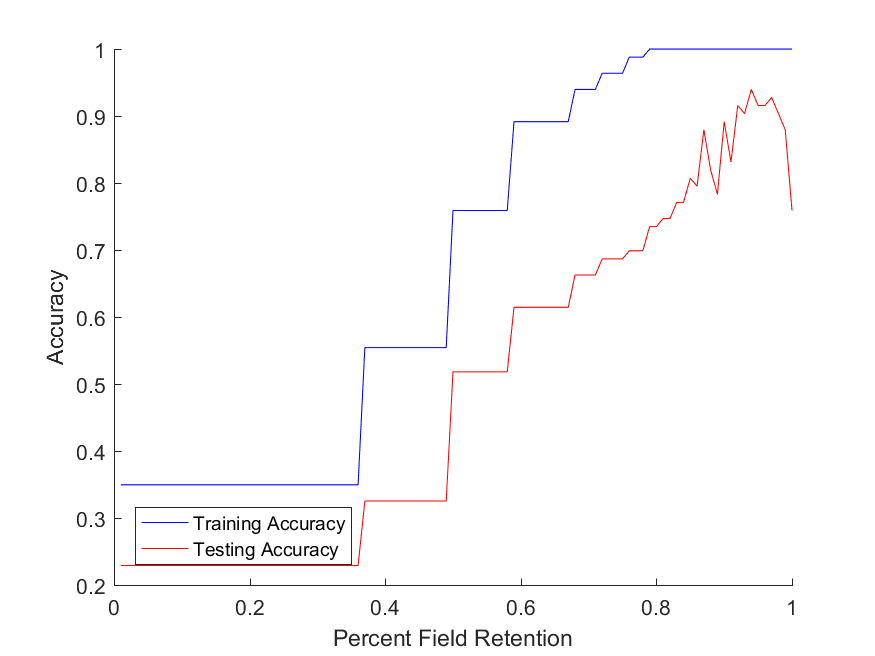
\includegraphics[width=115mm]{./accuracy_imgs/percent_field_retention_empirical.png}
    \captionof{figure}{Plot of accuracy as the field retention increases}
    \label{fig:img_size}
  \end{center}
\end{enumerate}

\newpage
\section{Optimally Trained Network}
Using the empirically investigated parameter values from the previous section we trained a network using the optimal values shown below.
\begin{center}
  \begin{table}[H]
    \begin{varwidth}[b]{0.4\linewidth}
      \centering
      \begin{tabular}{l|l}
        \hline
        Input layer bias node & Y \\
        Hidden layer bias node & N \\
        Standardization of features & Y \\
        PCA applied & Y \\
        \hline
        Training Iterations & 1000 \\
        Hidden Nodes & 1200 \\
        Image Size & 30 \\
        Learning Rate & 0.75 \\
        PCA Field Retention & 0.97 \\
        \hline
        Testing Accuracy & 0.8364 \\
        \hline
      \end{tabular}
      ~\\[40pt]
      \caption{Optimal Training Values}
      \label{table:optimal_table}
    \end{varwidth}%
    \hfill
    \begin{minipage}[b]{0.6\linewidth}
      \centering
      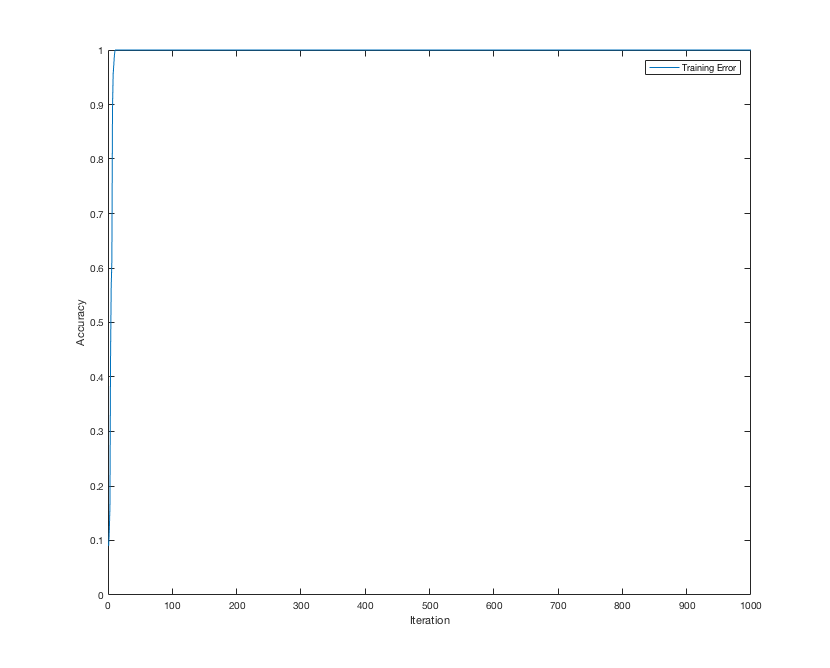
\includegraphics[width=100mm]{./accuracy_imgs/optimal_network.png}
      \captionof{figure}{Training Accuracy}
      \label{fig:optimal_plot}
    \end{minipage}
  \end{table}
\end{center}
Although the testing accuracy only increased from 0.8182 to 0.8364 the number of training iterations taken to reach 100\% training accuracy was decreased from 332 to 11.

\end{document}
